\section{Manual de usuario}\label{Manual usuario}

Para el correcto uso de la aplicación, el conjunto de acciones que se pueden realizar en dicho programa serán definidas a continuación. También, la distribución de las secciones de la interfaz junto a su explicación y funcionalidad.\bigskip

Cuando se ejecute el programa por primera vez en la pantalla se debe mostrar la siguiente interfaz de usuario:

\begin{figure}[!h]
    \centering
    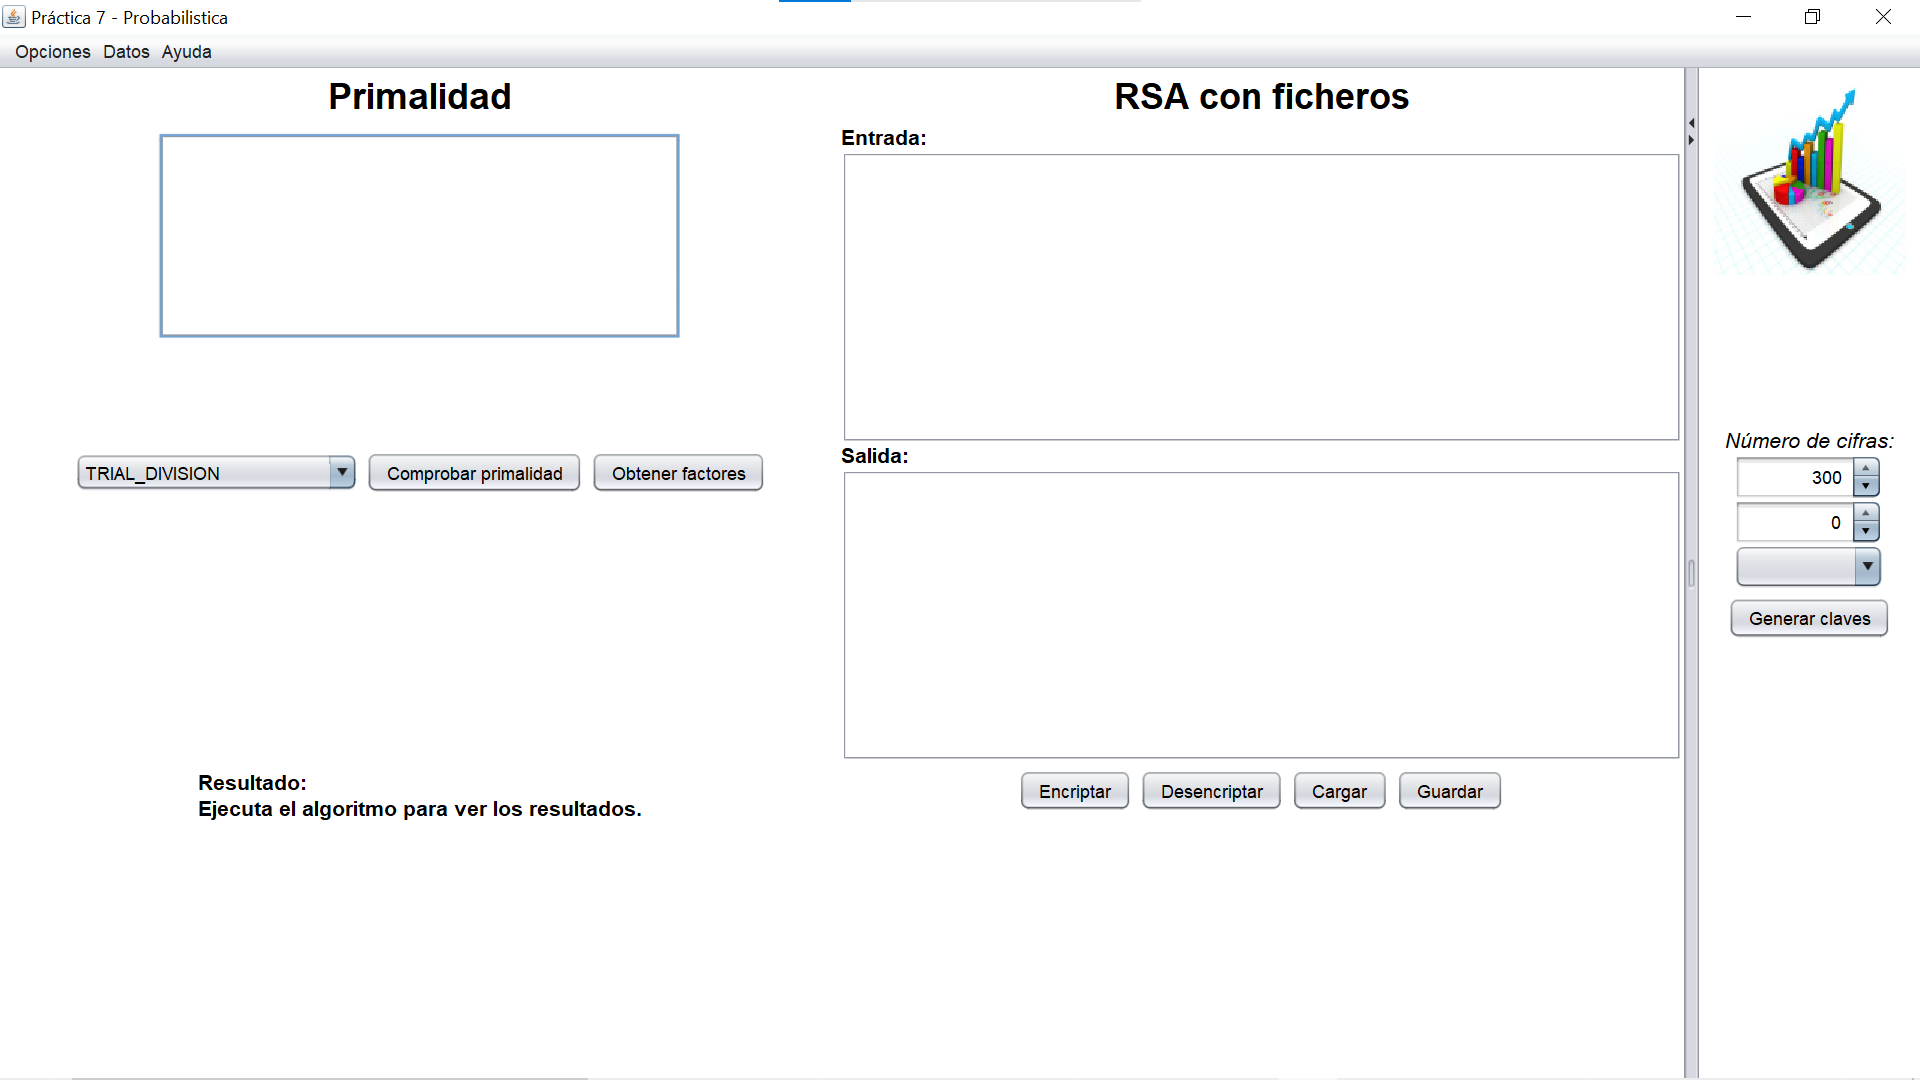
\includegraphics[width=\linewidth]{Usage/img/GUI.png}
    \caption{Interfaz de usuario.}
    \label{fig:User_interface}
\end{figure}

\subsection{Menu}\label{Manual usuario, Header}

El menú de la aplicación consiste en la barra que se sitúa debajo del marco superior de la ventana. En esta se puede encontrar un conjunto de opciones para que el usuario pueda interactuar con la aplicación, modificar y analizar el comportamiento de esta. En concreto, se encuentran las opciones de \say{Opciones}, \say{Datos} y \say{Ayuda}, respectivamente.\bigskip

En la primera se sitúan las acciones para salir del programa y para iniciar las ventanas de estadísticas explicadas anteriormente en los apartados \ref{Stats JVM} y \ref{Stats Algt}.\bigskip

En la segunda opción llamada \say{Datos} encontramos en primer lugar, la opción para crear una base de datos y cargar los datos. Por otra parte, tenemos la opción de obtener el resultado de la librería \say{Mesurament}.\bigskip

En la tercera opción se encuentra un menú desplegable con un manual de usuario con la explicación del funcionamiento de la aplicación.
 
\subsection{Main}

El \say{Main} es el bloque principal de la vista, donde el usuario podrá interactuar con múltiples opciones y apartados que se explicarán a continuación: \bigskip

En la parte izquierda tenemos el panel de \say{Primalidad}, aquí el usuario podrá introducir un número y comprobar si es primo con el botón de \say{Comprobar primalidad}. Bajo a éste se encuentra el botón \say{Obtener factores}, con el que se calculará la factorización del número introducido en el panel superior. Por otra parte, también se han añadido diferentes métodos de cálculo de primalidad en un selector, se han implementado los siguientes métodos:
\begin{itemize}
    \item Trial Division
    \item Fermat
    \item Miller Rabin
    \item Miller Rabin Parallel
    \item Trial Division Parallel
\end{itemize}
\bigskip

El resultado será mostrado por pantalla, además del tiempo que ha tardado en ser calculado. Si no se introduce un número, la aplicación avisará al usuario de que no es posible.\bigskip

En la parte derecha tenemos en panel de \say{RSA con ficheros}, con dos pequeños paneles, el superior \say{Entrada}, donde el usuario podrá introducir el texto. El panel inferior \say{Salida} será donde se generará el texto encriptado o desencriptado. Bajo a éste se encuentran los botones \say{Encriptar} y \say{Desencriptar} respectivamente. Además, se han añadido los siguientes botones, \say{Cargar} para cargar textos directamente y el botón \say{Guardar} para guardar la salida del texto.\bigskip

Cabe destacar que para encriptar o desencriptar el texto se deben usar las claves.

\subsection{Sidebar}\label{Sidebar}

El \say{Sidebar} contiene un conjunto de opciones para modificar los datos y el modo de ejecución de la aplicación. A continuación, se explicará cada una de estas opciones y su función.\bigskip

En primer lugar, se encuentra la opción para seleccionar el \say{Número de cifras}. En esta, se puede escoger el número de cifras para generar las claves.\bigskip

En segundo lugar, se encuentra un selector de las claves generadas y guardadas en base de datos. Tras clicar el botón \say{Cargar BD} del menú, se podrá seleccionar una key del selector. 

\subsection{Ejemplo ejecución}

Al iniciar la aplicación se mostrará una interfaz como la expuesta en la imagen \ref{fig:User_interface}. Por una parte, el usuario podrá introducir un número y calcular si es primo o sus factores. En el otro lugar, se podrá introducir un texto, y tras generar unas claves encriptar o desencriptar el texto. A continuación, la siguiente imagen, muestra un ejemplo de la interfaz tras la ejecución:

\begin{figure}[!h]
    \centering
    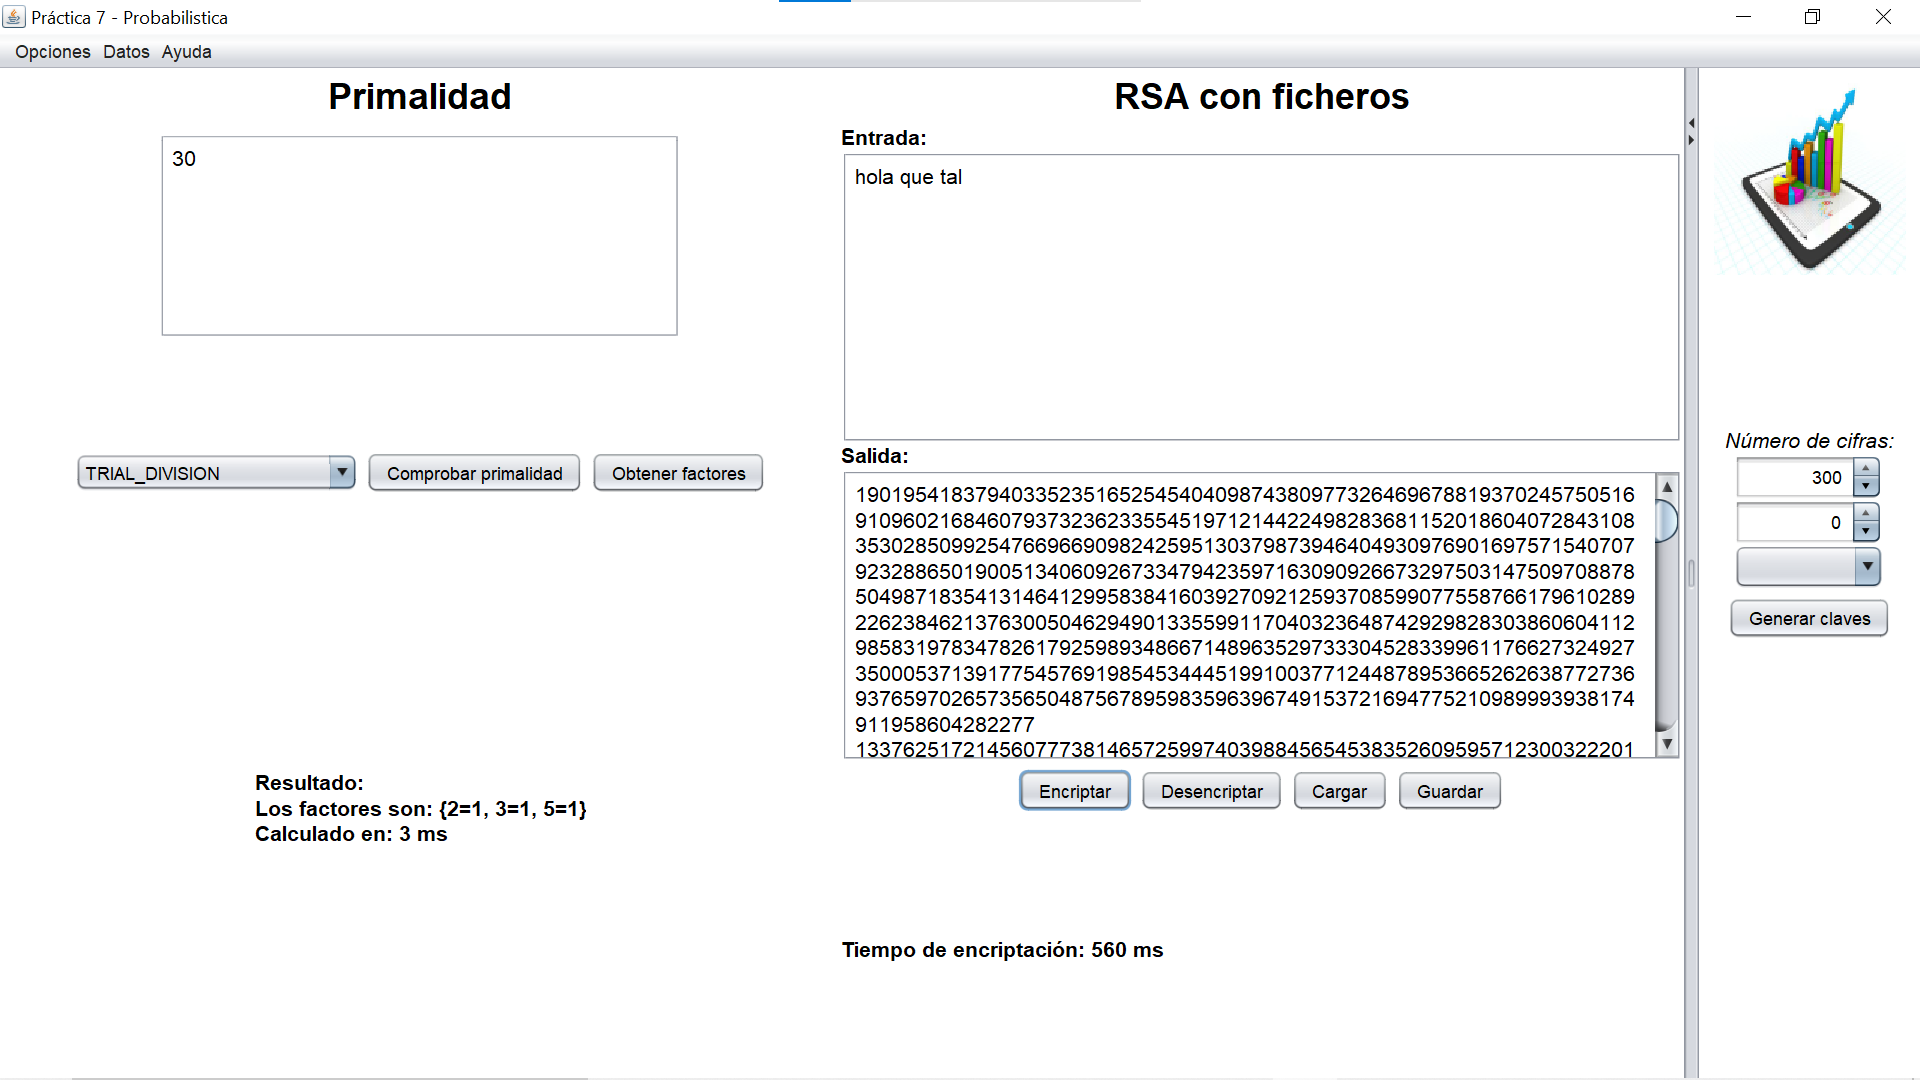
\includegraphics[width=\linewidth]{Usage/img/ejecucion.png}
    \caption{Interfaz de usuario en ejecución.}
    \label{fig:Ejemplo ejecución}
\end{figure}


A partir de aquí, el usuario puede salir del programa con el botón del menú, cargar una base de datos, mostrar el resultado de mesurament, calcular la primalidad o los factores de otro número, cambiar el método de primalidad, cambiar el número de cifras, encriptar o desencriptar texto y ver estadísticas de la ejecución, ver apartados \ref{Stats JVM} y \ref{Stats Algt}.
